% class
	% \documentclass[aspectratio = 169]{beamer} % 16:9
	\documentclass{beamer}
	\usetheme{Berlin}
	\definecolor{Main}{RGB}{150, 150, 150}
	\definecolor{DarkMain}{RGB}{100, 100, 100}
	\usecolortheme[named = Main]{structure}
	\usefonttheme{serif}

% packages
	% fonts
		\usepackage[T1]{fontenc}
		\usepackage[utf8]{inputenc}
	% math
		\usepackage{amsfonts}
		\usepackage{mathtools}
		\usepackage{bm}
	% pictures
		\usepackage{graphicx}
		\usepackage{subcaption}
		\usepackage{float}
		% tikz/pgf
			\usepackage{pgfplots}
			% warning!	
			% add several files with pgfplots raises the following error:
			%	TeX capacity exceeded, sorry [main memory size=3000000].
			% to solve it open a cmd and perform the following procedure:
			%	1. write
			%			initexmf --edit-config-file=pdflatex
			%	2. a text editor will open, add (or edit) the line 
			%			main_memory=12000000
			%	   then save and close the text editor
			%	3. write
			%			initexmf --dump=pdflatex
			%
			% source: https://florian-rappl.de/Articles/Page/239/latex-memory
				\def\mathdefault#1{#1}
				\everymath=\expandafter{\the\everymath\displaystyle}
				\makeatletter\@ifpackageloaded{underscore}{}{\usepackage[strings]{underscore}}\makeatother	
			\usepackage{tikz}
	% colors
		\usepackage{xcolor}
	% tables
		\usepackage{multirow}
	% algorithm
		\usepackage[ruled, vlined, linesnumbered]{algorithm2e}
		\usepackage{algorithmic}
		% remove algorithm header (default: "Algorithm 1:")
			\renewcommand{\algorithmcfname}{}
			\renewcommand{\thealgocf}{}
			\SetAlgoCaptionSeparator{}
	% itemize
		\usepackage{enumerate}
	% bibliography
		\usepackage[numbers]{natbib}
		\renewcommand{\bibname}{References}
		\renewcommand{\bibfont}{\footnotesize\interlinepenalty 10000\relax}
		\setlength{\bibsep}{1ex}
		\usepackage{doi}
	% other
		% boxes
			\usepackage{scalerel}
			\usepackage{adjustbox}
		% math
			\usepackage{transparent}
			\usepackage{cancel}
		% misc
			\usepackage{comment}	
			\usepackage{lipsum}
	
% setup
	% commands
		% external file of commands
			\usepackage{files/commands}
		% word spacing	
			\newdimen\origiwspc %
			\origiwspc = \fontdimen2\font % original inter word space
			\newcommand{\reducedspacing}[1]{\fontdimen2\font = 0.9\origiwspc #1 \fontdimen2\font = \origiwspc}
	% picutures
		\graphicspath{{./images/}}
		\pgfplotsset{compat = newest}
		% tikz
			\makeatletter
				\tikzset{
					dot diameter/.store in=\dot@diameter,
					dot diameter=3pt,
					dot spacing/.store in=\dot@spacing,
					dot spacing=10pt,
					dots/.style={
						line width=\dot@diameter,
						line cap=round,
						dash pattern=on 0pt off \dot@spacing
					}
				}
			\makeatother
	% adjust indentation
		\newlength\tindent
		\setlength{\tindent}{\parindent}
		\setlength{\parindent}{0pt}
		\renewcommand{\indent}{\hspace*{\tindent}}

% beamer preamble
	% remove beamer menu
		\beamertemplatenavigationsymbolsempty

	% layout
		% titlepage
			% parameters
				\def\thetitle{Generative Adversarial Nets}
				\def\thesubtitle{based on the original work of Goodfellow et al.}
				\def\theauthor{Francesco Caporali}
				\def\theinstitute{Department of Mathematics, University of Turin}
				\def\thedate{\today}
			% template		
				\title[\scshape{\thetitle}]{\large\scshape{\thetitle}}
				\subtitle{\texorpdfstring{\vspace{-0.3cm}\line(1, 0){200}\\\thesubtitle}{\thesubtitle}}
				\author[\scshape{\theauthor}]{\small\scshape{\theauthor}}
				\institute[\scshape{\thedate}]{\theinstitute}
				\date{\footnotesize\thedate}
				\newcommand{\firstpage}{
					\begingroup
						\setbeamertemplate{headline}{}
						\frame{
							\titlepage
						}
					\endgroup
				}
			% header/footer
				\setbeamertemplate{page number in head/foot}{\insertframenumber/\inserttotalframenumber}
				\setbeamertemplate{frametitle}{%
					\nointerlineskip%
					\begin{beamercolorbox}[wd = \paperwidth, ht = 2.4ex, dp = 1.1ex]{frametitle}
						\hspace*{1ex}\scshape\large{\insertframetitle}%
					\end{beamercolorbox}%
				}
				\setbeamertemplate{headline}{%
					\begin{beamercolorbox}[ht = 3.3ex, dp = 1.8ex]{section in head/foot}
						\scshape \insertsectionnavigationhorizontal{\textwidth}{}{}
					\end{beamercolorbox}%
				}
	% additional settings
		% transition transparency
			\setbeamercovered{transparent}
		% block colors
			\setbeamercolor{block title}{bg = Main}
			\setbeamercolor{alerted text}{fg = DarkMain}
		% wider slide	
			\newcommand\widerslide[2][3em]{
				\makebox[\linewidth][c]{
					\begin{minipage}{\dimexpr\textwidth+#1\relax}
						\raggedright#2
					\end{minipage}
				}
			}
			% mwe:
			% \begin{frame}
			% 	\widerslide[4em]{\lipsum[2]}
			% \end{frame}


\begin{document}

	\firstpage

	\section{Definitions}

	\begin{frame}
		The authors proposed a deep generative framework developed on a game theoretic idea. \\
		\medskip
		\textbf{Objective}: overcome the intractability issues of deep learning models that arises from conventional statistical approaches \\
		(e.g. maximum likelihood estimation). \\
		\medskip
		\textbf{Strategy}: 
		\begin{center}
			\begin{tabular}{ p{0.1\linewidth} | p{0.39\linewidth} | p{0.39\linewidth}}
				& \centering{Discriminator $D$} & \centering{Generator $G$} \tabularnewline [0.3cm]
				\multirow{2}{*}{\texttt{input}} & $z$: noise & \multirow{2}{*}{$z$: noise} \tabularnewline
				& $x$: sample data & \tabularnewline [0.3cm]
				\multirow{2}{*}{\texttt{goal}} & let $D(G(z))$ close to $0$, & generate $G(z)$, \tabularnewline
				& let $D(x)$ close to $1$ & let $D(G(z))$ close to $1$ 
			\end{tabular}
		\end{center}
	\end{frame}

	\begin{frame}
		Let $D$, $G$ be two maps generated through neural nets: \\
		\smallskip
		\hspace{20pt}\textit{Discriminator.} $D(x) \coloneqq D(x, \theta_D)$, $D: X \to [0, 1]$. \\
		\hspace{20pt}\textit{Generator.} $G(z) \coloneqq G(z, \theta_G)$, $G: Z \to X$; \\
		\medskip
		Given $x \in X$ (data space), $z \in Z$ (noise space), we define:
		\begin{itemize}
			\item[-] $p_\text{\texttt{data}}(x)$, density of the input data;
			\item[-] $p_G(x)$, density of the Generator;
			\item[-] $p_\text{\texttt{noise}}(z)$, density of a prior noise. 
		\end{itemize}
		\vspace{-0.2cm}
		\begin{center} \line(1, 0){200} \end{center}
		\vspace{-0cm}
		$D$ and $G$ play a minimax game with value function $V(D, G)$,
		\begin{equation*}
			V(D, G) \coloneqq \mean[x \sim p_\text{\texttt{data}}]{\log{D(x)}} + \mean[z \sim p_\text{\texttt{noise}}]{\log{1 - D(G(z))}}.
		\end{equation*}
		We aim to find $D^*, G^*$ s.t. $V(D^*, G^*) = \min_G \max_D \ V(D, G)$.
	\end{frame}

	\begin{frame}
		\begin{center} \textbf{Discriminator goal} \end{center}
		\begin{equation*}
			\max_{D} \ \underbrace{\mean[x \sim p_\text{\texttt{data}}]{\log{D(x)}}}_{D(x) \ \approx \ 1} + \underbrace{\mean[z \sim p_\text{\texttt{noise}}]{\log{1 - D(G(z))}}}_{D(G(z)) \ \approx \ 0}.
		\end{equation*}
		\begin{center} \textbf{Generator goal} \end{center}
		\begin{equation*}
			\min_{G} {\transparent{0.3}{\max_{D}}} \ \cancel{\mean[x \sim p_\text{\texttt{data}}]{\log{D(x)}}} + \underbrace{\mean[z \sim p_\text{\texttt{noise}}]{\log{1 - D(G(z))}}}_{D(G(z)) \ \approx \ 1}.
		\end{equation*}
		\begin{block}{Remark}
			Under the (unrealistic) assumption of being able to find the optimal discriminator $D^*_G \coloneqq \max_{D} V(D, G)$, it is possible to show that iteratively alternating computations of $D^*_G$ and updates of $G$ (to minimize $V(D^*_G, G)$), one would obtain $p_G = p_{\text{\texttt{data}}}$.
		\end{block}
	\end{frame}
	
	% Note:
	% As remarked, the unrealistic assumption of finding the optimal discriminator is solved in practical implementations. Instead we proceed alternating k optimization steps of D with 1 optimization step of G. This is similar to what happens when we implement Markov Chains algorithms, in this way it is possible to let the sampling distribution p_G to slowly converge to the stationary distribution of the chain.

	\section{Theoretical guarantees}

	\begin{frame}
		\begin{block}{Proposition 1 \hfill [\citeauthor{goodfellow2014}]}
			For a fixed generator $G$, the associated optimal discriminator $D^*_G$ is
			\vspace{-0.3cm}
			\begin{equation*}
				D^*_G(x) = \frac{p_{\text{\texttt{data}}}(x)}{p_{\text{\texttt{data}}}(x) + p_G(x)}, \, \forall x \in X.
			\end{equation*}		
		\end{block}
		\textit{Proof.} 
		\begin{enumerate}
			\item 
				Thanks to the Radon-Nikodym Theorem we have 
				\vspace{-0.2cm}
				\begin{equation*}
					\mean[z \sim p_\text{\texttt{noise}}]{\log{1 - D(G(z))}} = \mean[x \sim p_G]{\log{1 - D(x)}}.
				\end{equation*}
			\item 
				Hence we can rewrite $V(D, G)$ as
				\vspace{-0.3cm}
				\begin{equation*}
					V(D, G) = \int_X \log{D(x)} p_\text{\texttt{data}}(x) + \log{1 - D(x)} p_G(x) dx, 
				\end{equation*}
				\vskip -0.3cm
				with $\supp{p_G} = G(\supp{p_\text{\texttt{noise}}}) \subset X$, $\supp{p_\text{\texttt{data}}} \subset X$.
		\end{enumerate}
	\end{frame}

	\begin{frame}
		\begin{enumerate}\setcounter{enumi}{2}
			\item 
				Consider $f: [0, 1] \to \real$, $f(y) \coloneqq \log{y} a + \log{1 - y} b$, with $a, b > 0$, then $f$ is a concave map and the only maximum is realized by $y = \frac{a}{a + b}$.
			\item 
				Defining $\tilde{D} \coloneqq \frac{p_\text{\texttt{data}}}{p_\text{\texttt{data}} + p_g}$, we have, by monotonicity of the integral, $\forall D$,
				\vspace{-0.2cm}
				\begin{align*}
					& V(D, G) \kern-1pt = \kern-2pt \int_X \kern-2pt \log{D(x)} p_\text{\texttt{data}}(x) \kern-2pt + \kern-2pt \log{1 \kern-2pt - \kern-2pt D(x)} p_G(x) dx \leq \\
					& \leq \kern-3pt \int_X \kern-2pt \log{\kern-2pt \tilde{D}(x) \kern-2pt} p_\text{\texttt{data}}(x) \kern-2pt + \kern-2pt \log{\kern-2pt 1 \kern-2pt - \kern-2pt \tilde{D}(x) \kern-2pt} p_G(x) dx \kern-2pt = \kern-2pt V(\tilde{D}, G),
				\end{align*}
				$\implies \tilde{D} = \argmax_{D} V(D, G) = D^*_G$.
		\end{enumerate}
		\qed
	\end{frame}

	\begin{frame}
		\begin{block}{Theorem 1 \hfill [\citeauthor{goodfellow2014}]}
			The global minimum of the virtual training criterion given by $C(G) \coloneqq \max_D V(D, G)$, is achieved if and only if $p_G = p_\text{\texttt{data}}$. \\ 
			For such minimum $G$, $C(G) = -\log{4}$.
		\end{block}
		\textit{Proof.} 
		\begin{enumerate}
			\item Let us first rewrite the criterion in a more suitable way:
				\vspace{-0.2cm}
				\begin{align*}
					C(G) & = V(\argmax_D V(D, G), G) = V(D^*_G, G) = \\
					& = \mean[x \sim p_\text{\texttt{data}}]{\log{D^*_G(x)}} + \mean[z \sim p_G]{\log{1 - D^*_G(x)}} = \\
					& = \mean[x \sim p_\text{\texttt{data}}]{\log{\frac{p_\text{\texttt{data}}(x)}{p_\text{\texttt{data}}(x) + p_G(x)}}} + \\
					& \kern12.2pt + \mean[z \sim p_G]{\log{\frac{p_G(x)}{p_\text{\texttt{data}}(x) + p_G(x)}}}.
				\end{align*}
		\end{enumerate}
	\end{frame}

	\begin{frame}
		\begin{enumerate}\setcounter{enumi}{1}
			\item Let $\tilde{G}$ be a generator such that $p_{\tilde{G}} = p_\text{\texttt{data}}$, then $C(\tilde{G}) = 2 \log{1/2} = -\log{4}$.
			\item Morever, adding and subtracting $-\log{4}$, we have that
				\vspace{-0.2cm}
				\begin{equation*}
					C(G) = -\log{4} + 2 \jsd{p_\text{\texttt{data}} \,\|\, p_G}, \, \forall G.
				\end{equation*}
			\item We recall the properties of the Jensen-Shannon divergence: $\forall p, q$ densities $\jsd{p \,\|\, q} \geq 0$ and $\jsd{p \,\|\, q} = 0$ if and only if $p = q$.
			\item Those properties are sufficient to conclude that 
				\vspace{-0.2cm}
				\begin{gather*}
					\min_G C(G) = -\log{4} \text{ and} \\
					C(G) = -\log{4} \iff p_\text{\texttt{data}} = p_G.
				\end{gather*}
		\end{enumerate}
		\qed
	\end{frame}

	\begin{frame}
		\begin{block}{Proposition 2 \hfill [\citeauthor{goodfellow2014}]}
			If $G$ and $D$ have enough capacity, and at each iteration of the algorithm, $D$ reaches its optimum given $G$, and $p_G$ is updated so as to improve the criterion
			\vspace{-0.3cm}
			\begin{equation*}
				\mean[x \sim p_\text{\texttt{data}}]{\log{D^*_G(x)}} + \mean[z \sim p_G]{\log{1 - D^*_G(x)}}
			\end{equation*}
			\vskip -0.3cm
			then $p_G$ converges to $p_\text{\texttt{data}}$.
		\end{block}
		\textit{Sketch.} 
		\begin{enumerate}
			% x = G, \beta = D^*_{G_\text{old}} (in paper notation)
			\item $f(G) \coloneqq \max_D V(D, G)$, $f_{D^*_{G_\text{old}}}(G) \coloneqq V(D^*_{G_\text{old}}, G)$, with $G_\text{old}$ which is the resulting generator after its last update.
			\item We would like to update $G$ descending the stochastic gradient of $f$ because this would mean that $p_G$ is closer to $p_\text{\texttt{data}}$ than $p_{G_\text{old}}$ was.
		\end{enumerate}
	\end{frame}
	
	\begin{frame}
		\begin{enumerate}\setcounter{enumi}{2}
			\item However this is equivalent to update $G$ descending the stochastic gradient of $f_{D^*_{G_\text{old}}}$ (which is what we do). \\
			This assertion follows from the fact that the subgradients of $f_{D^*_{G_\text{old}}}$ are a subset of the subgradients of $f$: $\partial f_{D^*_{G_\text{old}}} \subset \partial f$ (from the convexity of $V(D, G)$).
		\end{enumerate}
		\begin{block}{Remark}
			Note that the algorithm used to train the GANs does not optimize the underlying distribution of $G$, $p_G$, but the parameters of a neural net, $\theta_G$. \\
			\medskip
			This raises theoretical problems, anyway the performances of the model are impressive, therefore GANs are reasonable to be used in practice.
		\end{block}
	\end{frame}

	
	\section{Training}

	\begin{frame}
		\SetNlSty{texttt}{}{.}
		\SetAlgoNlRelativeSize{-1}
		\setlength{\algomargin}{2em}
		\begin{algorithm}[H]
			% caption
			\caption{\vspace{-0.07cm}\textbf{Algorithm.} Minibatch SGD for training $D$ and $G$}
			% format
			\DontPrintSemicolon
			\SetKwBlock{Function}{function}{end function}
			% algorithm
			\Function($\textit{\texttt{train}}{(D, G, \textit{\texttt{data}}, k, \textit{\texttt{n\_epochs}})}$){
				\For{$\texttt{epoch} \textnormal{\textbf{ in }} 1, \dots, \texttt{n\_epochs}$}
				{
					\For{$\_ \textnormal{\textbf{ in }} 1, \dots, k$}
					{
						sample $\mathbf{z} = (z_i)_{i = 1}^{m}, \, z_i \sim p_{\texttt{noise}}$ \;
						sample $\mathbf{x} = (x_i)_{i = 1}^{m}, \, x_i \sim p_{\texttt{data}}$ \;
						$\theta_D = \theta_D + \lambda \, \nabla_{\theta_D} \widehat{V}_m(D, G)$ \;
					}
				sample $\mathbf{z} = (z_i)_{i = 1}^{m}, \, z_i \sim p_{\texttt{noise}}$ \;
				$\theta_G = \theta_G - \lambda \, \nabla_{\theta_G} \widehat{V}_m(D, G)$ \;
				}
				\Return{D, G}
			}
		\end{algorithm}
		\medskip 
		Where the sample mean of the loss $V(D, G)$ is computed on the $m$-dimensional minibatches $\mathbf{z}, \mathbf{x}$:
		\vspace{-0.2cm}
		\begin{equation*}
			\widehat{V}_m(D, G) \coloneqq \frac{1}{m} \sum_{i = 1}^{m} \log{D(x_i)} + \frac{1}{m} \sum_{i = 1}^{m} \log{1 - D(G(z_i))}.
		\end{equation*}
	\end{frame}

	\begin{frame}
		\begin{block}{Remark}
			Actual implementation:
			\begin{itemize}
				\item[-] 
					{\color{Main}{\textit{$6$\textsuperscript{th} line.}}} It is performed one step of the ascent of the stochastic gradient via backpropagation, with loss 
					\vspace{-0.3cm}
					\begin{equation*}
						\widehat{V}_m(D {\transparent{0.3}{, G}}) = \frac{1}{m} \sum_{i = 1}^{m} \log{D(x_i)} + \log{1 - D(G(z_i))};
					\end{equation*}
					\vspace{-0.6cm}
				\item[-] 
				{\color{Main}{\textit{$8$\textsuperscript{th} line.}}} Instead of one step of the ascent of $\widehat{V}_m({\transparent{0.3}{D,}} \, G)$ we, equivalently, do a step of descent with loss 
					\vspace{-0.3cm}
					\begin{equation*}
						\frac{1}{m} \sum_{i = 1}^{m} \log{D(G(z_i))};
					\end{equation*}
			\end{itemize}
			\textit{Note.} The classical SGD is often substituted by SGD with momentum or adaptative algorithm (like ADAM).
		\end{block}
	\end{frame}

	\section{Simulations}

	\begin{frame}
		We performed practical simuations, training and generating data using GANs (based on the work of \citeauthor{vandegarweb}). \\
		\medskip
		The dataset used as train set is \texttt{MNIST}, a database of $60000$ images of handwritten digits.
		\begin{figure}[H]
			\begin{center}
				% [trim = {left bottom right top}, clip]
				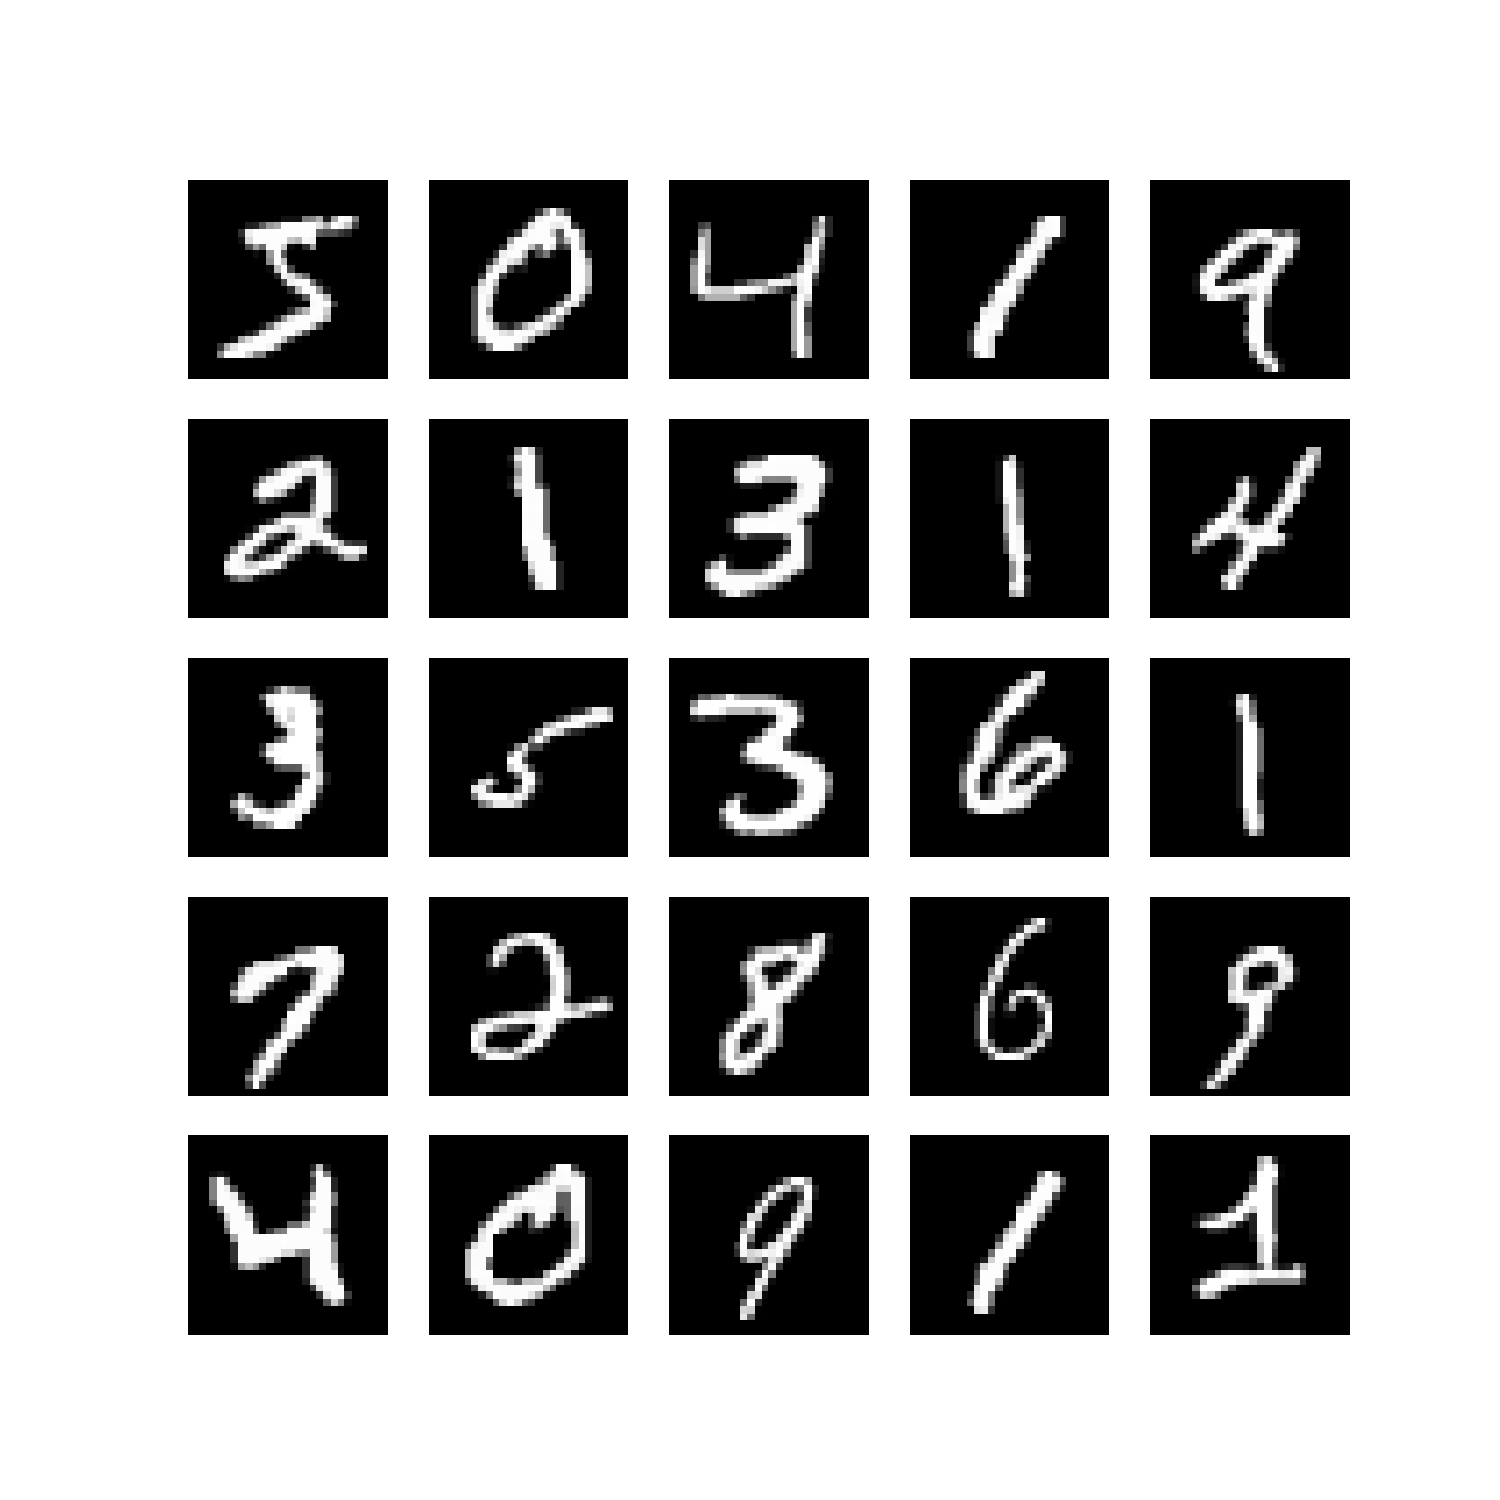
\includegraphics[scale = 0.28, trim = {0 3cm 0 3cm},clip]{head_mnist_data.pdf}
			\end{center}
		\end{figure}
	\end{frame}

	\begin{frame}
		\vspace{0.3cm}
		Generated samples obtained after $10^{4}$ and $10^{5}$ epochs of training using nets $D$, $G$ with architectures $\alpha_D$, $\alpha_G$:
		\vspace{-0.1cm}	
		\begin{align*}
			\alpha_D &= \big((28 \times 28, 240, 240, 1), (\activation{LeakyReLU}, \activation{LeakyReLU}, \activation{Sigmoid})\big), \\
			\alpha_G &= \big((100, 1200, 1200, 28 \times 28), (\activation{ReLU}, \activation{ReLU}, \activation{Tanh})\big).
		\end{align*}
		\vspace{-0.5cm}
		\begin{figure}[H]
			\begin{center}
				% [trim = {left bottom right top}, clip]
				\begin{subfigure}{0.45\textwidth}
					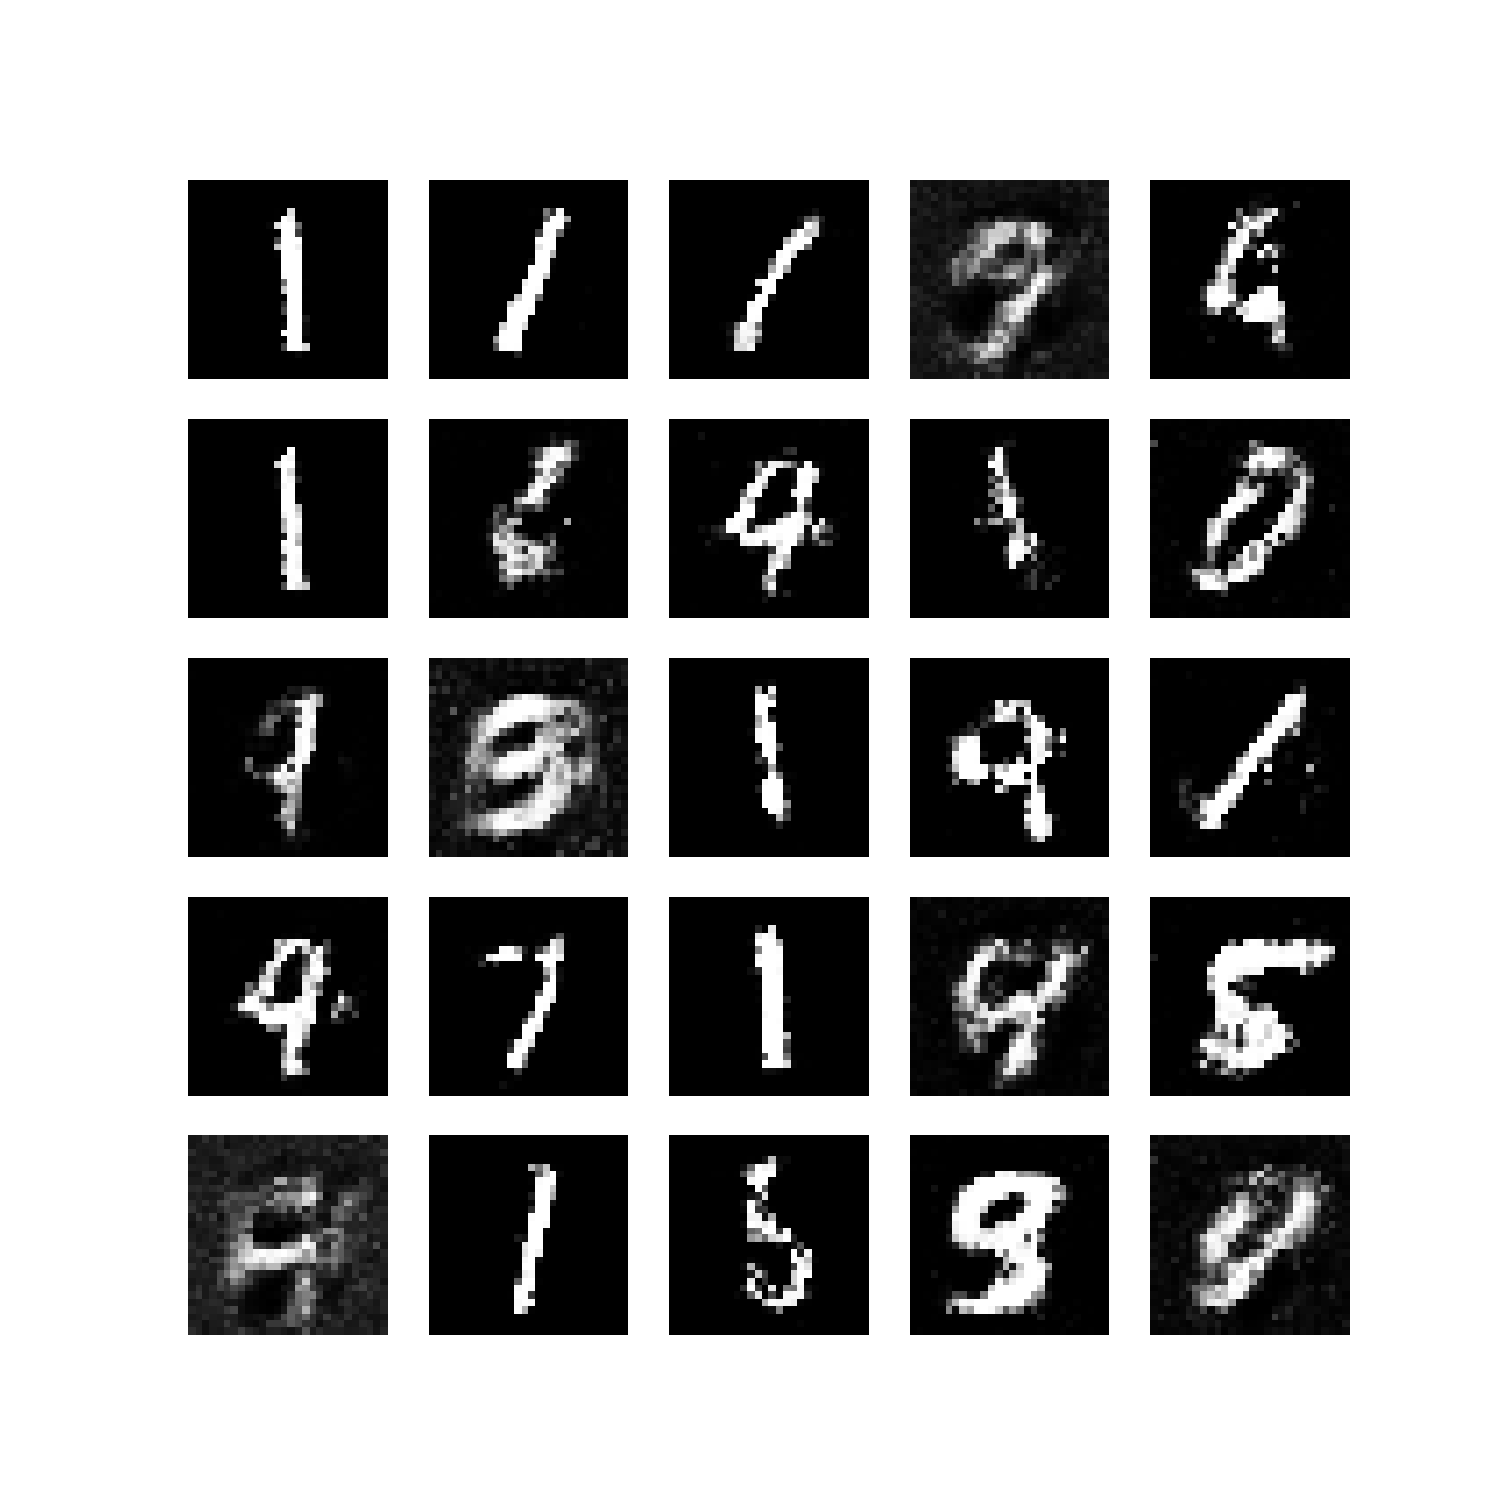
\includegraphics[scale = 0.23, trim = {3cm 3cm 3cm 3cm},clip]{regenerated_mnist_data_10000.pdf}
					\caption{$10^{4}$ epochs}
				\end{subfigure}
				\hspace{0.2cm}
				\begin{subfigure}{0.45\textwidth}
					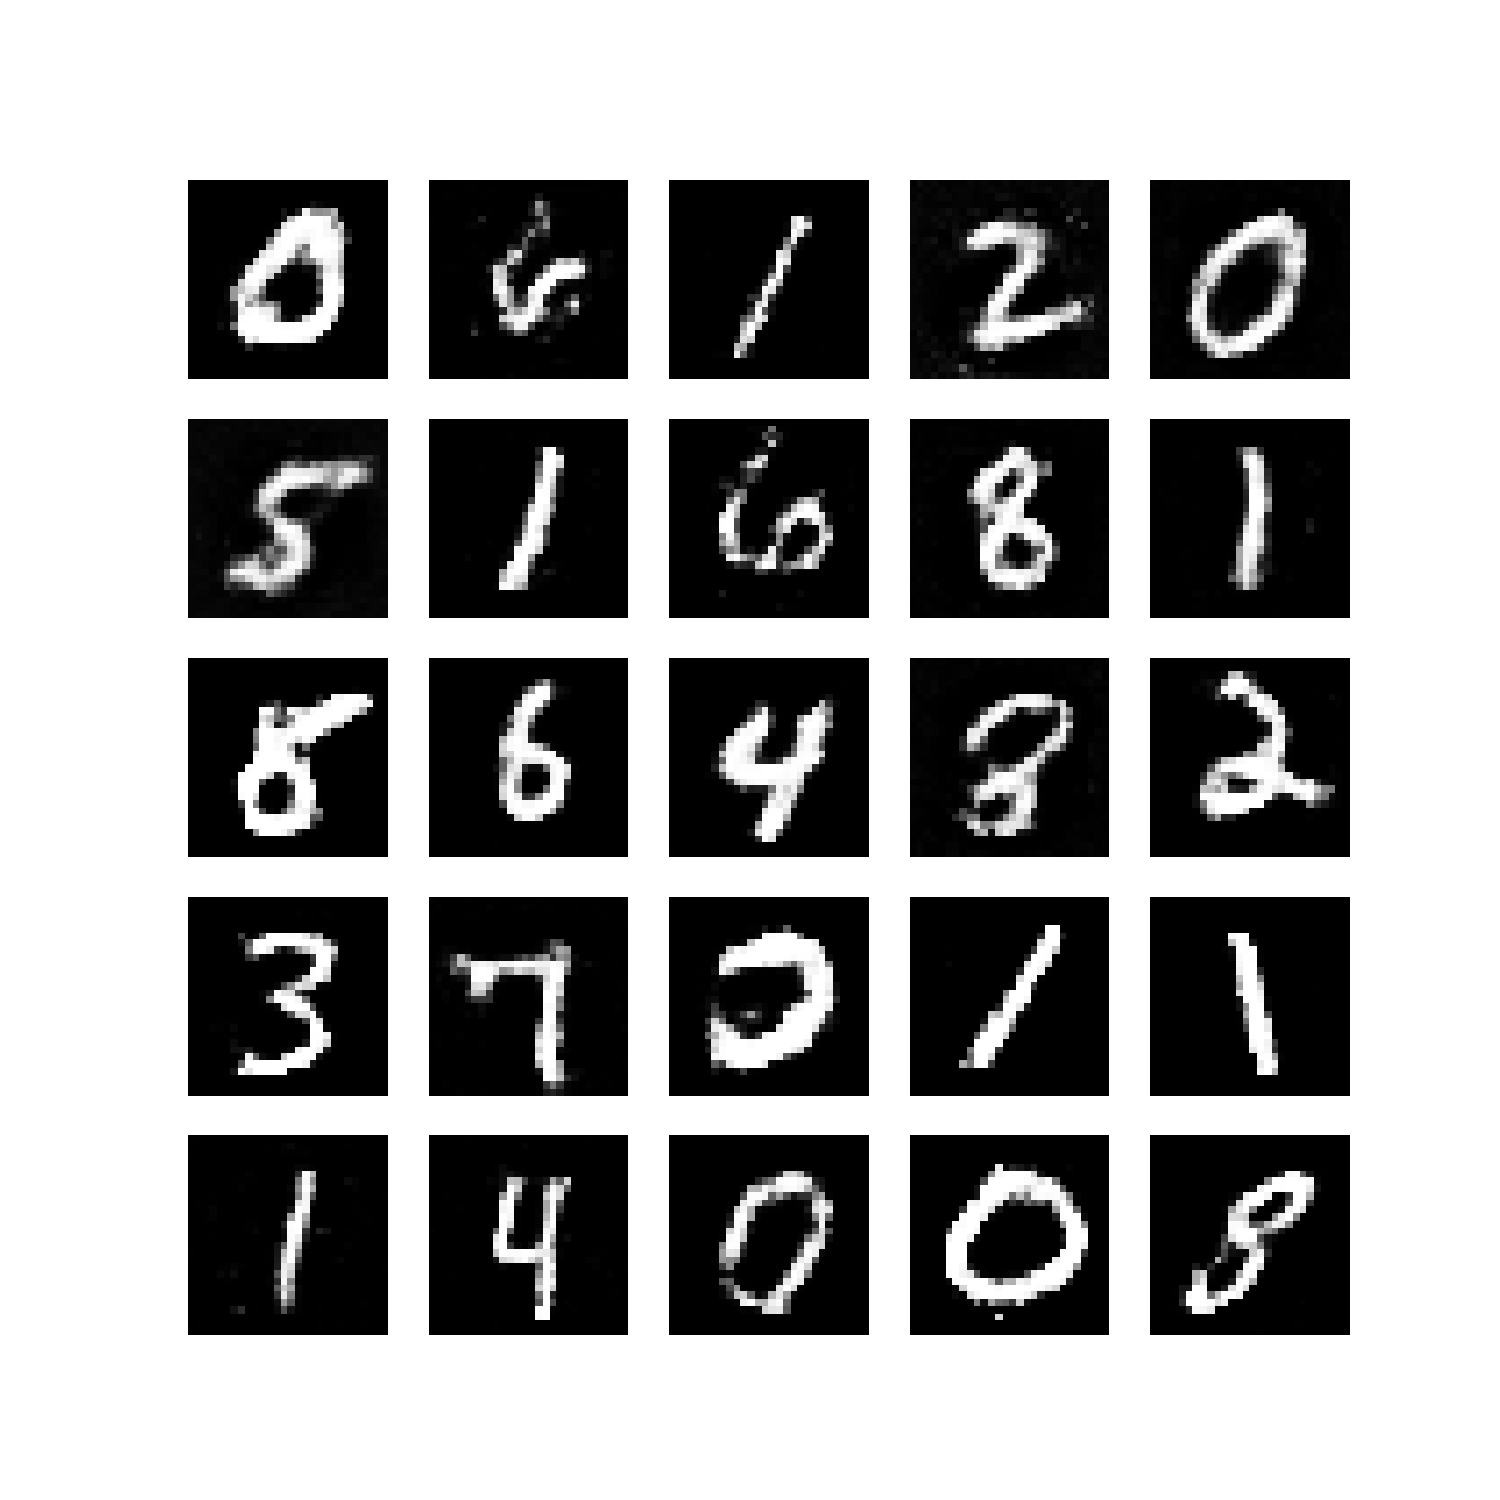
\includegraphics[scale = 0.23, trim = {3cm 3cm 3cm 3cm},clip]{regenerated_mnist_data_100000.pdf}
					\caption{$10^{5}$ epochs} 
				\end{subfigure}
			\end{center}
		\end{figure}
	\end{frame}
	
	% bibliography
	\begin{frame}%[allowframebreaks]
		\frametitle{\textsc{References}}
		\nocite{*} 
		\bibliographystyle{plainnat}
		\bibliography{files/bibliography}
	\end{frame}

\end{document}